\documentclass[11pt]{article}
\usepackage[left=3.5cm,right=3.5cm,top=2.5cm,bottom=2.5cm]{geometry}
%\usepackage[spanish]{babel}
\overfullrule = 5mm

\usepackage{amsmath,amsfonts,amsthm}
\usepackage{enumitem,mathtools,graphicx}
\setenumerate[0]{label=(\alph*)}

\newtheorem{definition}{Definición}
\newtheorem{reminder}{Recordatorio}
\newtheorem{exercise}{Ejercicio}
\newtheorem*{sol}{Solución}
\newtheorem*{theorem}{Teorema}

\newcommand\N{\mathbb N}
\newcommand\R{\mathbb R}
\newcommand\C{\mathbb C}
\newcommand\ol\overline

\usepackage{csquotes}
\usepackage[style=authoryear]{biblatex}
\addbibresource{references.bib}

\title{Análisis numérico para ecuaciones diferenciales \\
Tarea 3 - Métodos Runge-Kutta}
\author{Jorge Alfredo Álvarez Contreras}

\begin{document}
\maketitle

\begin{reminder}
  El método asociado al tablero de Butcher
  \begin{equation}
    \begin{array}{c|c}
      c & A \\
      \hline \\[-3mm]
        & b^T
    \end{array}
  \end{equation}
  es
  \begin{equation}\label{eq:metodomultipaso}
    u_{n+1} = u_n + h F(t_n,u_n,h,f),
  \end{equation}
  donde
  \begin{align}
    F
      &= \sum_{i=1}^{s}b_ik_i
      \\[-3mm]
    k_i
      &= f(t_n+c_ih, u_n+h \sum_{j=1}^{s}a_{ij} k_j)
      \\[-4mm]
    \text{y} \quad
    c_i
      &= \sum_{j=1}^{s}a_{ij}
  .\end{align}
\end{reminder}

\begin{reminder}
  Para analizar la estabilidad absoluta del método
  \eqref{eq:metodomultipaso}, lo aplicamos al problema de prueba
  $f(t,y)=\lambda y$, con lo que obtenemos
  \begin{align}
    k_i
    &= \lambda(u_n+h \sum_{j=1}^{s}a_{ij} k_j) \\
    &= \lambda u_n+z \sum_{j=1}^{s}a_{ij} k_j
  .\end{align}
  Ahora definimos $K$ como la columna formada por los $k_i$. Es decir,
  \begin{align}
    K = \lambda u_n\bar 1+zAK
  ,\end{align}
  donde $\bar 1$ es una columna cuyas entradas son todas iguales a
  $1$. Despejando $K$, esto es
  \begin{equation}
    K=\lambda (I-zA)^{-1}u_n\bar 1
  .\end{equation}
  Por lo tanto, $F=b^{T}K$ y
  \begin{align}
    u_{n+1}
    &= u_n + hF(t_n,u_n,h,f) \\
    &= u_n + hb^TK \\
    &= u_n + h\lambda b^T(I-zA)^{-1}u_n\bar 1 \\
    &= u_n[1 + h\lambda b^T(I-zA)^{-1}\bar 1]
  .\end{align}
  La función de estabilidad del método es la función
  $R(z)=R(h\lambda)$ dentro del corchete, i.e.
  \begin{equation}
    R(z) = 1 + zb^T(I-zA)^{-1}\bar 1
  .\end{equation}
\end{reminder}

\section{Ejercicios}

\begin{exercise}
   Programar el método Runge-Kutta Fehlberg para resolver el problema
   de valores iniciales
   \begin{equation}
     y'
     =
     (1-2x)y,
     \quad y(0)=1,
     \quad 0\leq x\leq 4
   ,\end{equation}
   tomando $h_\mathrm{max}=0.1$ y tolerancia $\epsilon = 0.01$.
   Elaborar una gráfica del error y una gráfica de $x_n$ contra $h_n$.
   (Marque con un punto los pasos aceptados y con un asterisco los
   pasos rechazados).
\end{exercise}
\begin{sol}
  Se incluye una gráfica de la solución obtenida:
  \begin{center}
  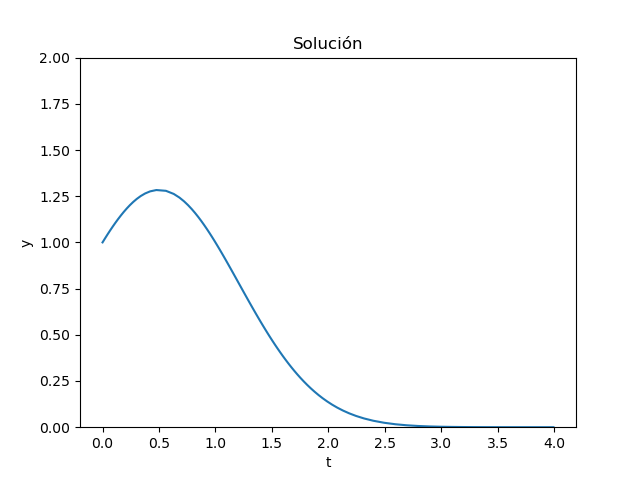
\includegraphics[width=0.9\textwidth]{img/jaac_tarea3_ejercicio1a}
  \end{center}
  \newpage
  El error se comporta como sigue:
  \begin{center}
  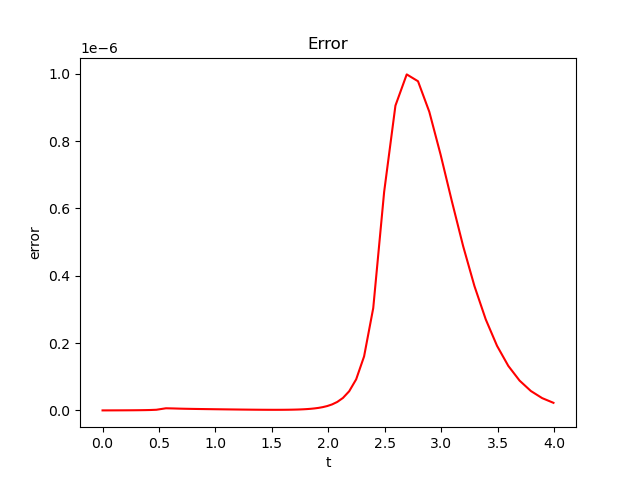
\includegraphics[width=0.9\textwidth]{img/jaac_tarea3_ejercicio1b}
  \end{center}
  Finalmente, se ilustran los tamaños de paso intentados en cada punto
  del tiempo $t$. Las cruces son rechazos de tamaño de paso y los
  puntos indican cuando el tamaño de paso produce una aproximación que
  pasa la tolerancia.
  \begin{center}
  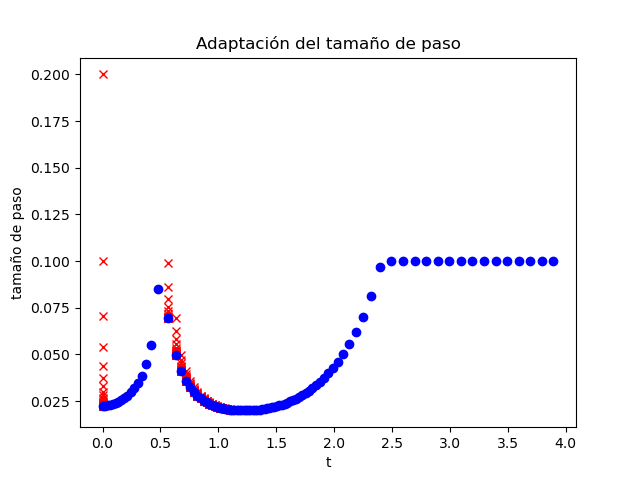
\includegraphics[width=0.9\textwidth]{img/jaac_tarea3_ejercicio1c}
  \end{center}
\end{sol}

\newpage

\begin{exercise}
  Considere la familia de métodos de Runge-Kutta correspondientes al
  table\-ro de Butcher
  \begin{equation}
    \begin{array}{c|cc}
      0 & 0 & 0 \\
      \frac{1}{2\theta} & \frac{1}{2\theta} & 0 \\[2mm]
      \hline \\[-3mm]
                        & 1-\theta & \theta.
    \end{array}
  \end{equation}
  Determine el orden del método y la función de estabilidad
  $R(h\lambda)$. Elabore una gráfica de la región de estabilidad
  absoluta.
\end{exercise}
\begin{sol}
  Para el tablero de Butcher del problema, tenemos
  \begin{align}
    F
      &= (1-\theta)k_1 + \theta k_2, \\
    k_1
      &= f(t_n, u_n) \\
      &= f_n \\
    k_2
      &= f(t_n+\tfrac{h}{2\theta}, u_n+\tfrac{h}{2\theta}k_1) \\
      &= f(t_n+\tfrac{h}{2\theta}, u_n+\tfrac{h}{2\theta}f_n),
  \end{align}
  así que
  \begin{align}
    u_{n+1}
    &= u_n + hF \\
    &= u_n + h[(1-\theta)k_1 + \theta k_2] \\
    &= u_n + h[(1-\theta)f_n
    + \theta f(t_n+\tfrac{h}{2\theta}, u_n+\tfrac{h}{2\theta}f_n)].
  \end{align}
  Notemos que este método es de la forma
  \begin{equation}
    u_{n+1}
    = u_n + h[af(t_n,u_n) + bf(t_n+\alpha h, u_n+\beta h f_n)]
  \end{equation}
  con $a+b=1$ y $\alpha=\beta=\frac{1}{2b}$, donde $b=\theta$. En el
  problema 5 de la tarea 1 probamos que este método es de orden $2$.
  La función de estabilidad es 
  \begin{align}
    R(z)
    &= 1 + zb^T(I-zA)^{-1}\bar 1 \\
    &= 1 + z
      \begin{bmatrix}
        1-\theta & \theta
      \end{bmatrix}
      \begin{bmatrix}
        1 & 0 \\
        -\frac{z}{2\theta} & 1
      \end{bmatrix}
      \begin{bmatrix}
        1 \\ 1
      \end{bmatrix}
    \\
    &= 1 + z
      \begin{bmatrix}
        1-\theta & \theta
      \end{bmatrix}
      \begin{bmatrix}
        1 & 0 \\
        \frac{z}{2\theta} & 1
      \end{bmatrix}
      \begin{bmatrix}
        1 \\ 1
      \end{bmatrix}
    \\
    &= 1 + z
      \begin{bmatrix}
        1-\theta & \theta
      \end{bmatrix}
      \begin{bmatrix}
        1 \\
        \frac{z}{2\theta} + 1
      \end{bmatrix}
    \\
    &= 1 + z[(1-\theta)+\theta(\tfrac{z}{2\theta}+1)] \\
    &= 1 + z(1+\tfrac{z}{2}) \\
    &= 1 + z+\frac{z^{2}}{2}
  .\end{align}
  Esta es la misma función de estabilidad que la del problema 2
  (inciso (a)) de la tarea 2. Por lo tanto, obtenemos la misma
  gráfica de la región de estabilidad $|R(z)|<1$:
   \begin{center}
  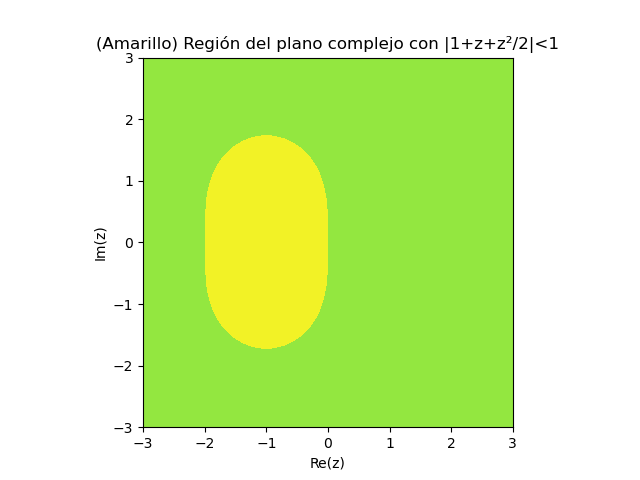
\includegraphics[width=0.8\textwidth]{img/jaac_tarea2_ejercicio2a}
  \end{center}
\end{sol}

\begin{exercise}
  Considere el método de Runge-Kutta con tablero de Butcher dado por
  \begin{equation}
    \begin{array}{c|c}
      c & A \\
      \hline \\[-3mm]
        & b^T
    \end{array}
  \end{equation}
  donde $A$ es una matríz estrictamente triangular inferior. Demuestre
  que $R(h\lambda)$ es el polinomio en $z=h\lambda$ dado por 
  \begin{equation}\label{eq:estabilidad_alt}
    R(z) = \det(I-zA+z\ol 1 b^T)
  .\end{equation}
\end{exercise}
\begin{sol}
  Debemos mostrar que la función de estabilidad
  \begin{equation}
    R(z) = 1 + zb^T(I-zA)^{-1}\bar 1
  \end{equation}
  es equivalente a la expresión \eqref{eq:estabilidad_alt}.
  La siguiente demostración está sacada de
  \cite[p.213]{butcher2004numerical}.
  Sean $v$ un vector de $n$ entradas y $v'$ el vector de $n-1$
  entradas que se obtiene eliminando la primera entrada de $v$ y
  denotemos como $I'$ a la matríz identidad de $(n-1)\times(n-1)$.
  También denotemos $\ol 1'$ como el vector de $n-1$ entradas formado
  por unos. Entonces la matríz $\ol 1v^{T}$ tiene polinomio
  característico
  \begin{align}
    \chi(x)
    &= 
    \det(xI - \ol 1 v^T) \\
    &= \det
    \begin{bmatrix}
      x-v_1 & -v_2 & -v_3 & \cdots & -v_n \\
      -v_1 & x-v_2 & -v_3 & \cdots & -v_n \\
      -v_1 & -v_2 & x-v_3 & \cdots & -v_n \\
      \vdots & \vdots & \vdots & \ddots & \vdots \\
      -v_1 & -v_2 & -v_3 & \cdots & x-v_n \\
    \end{bmatrix}
    \\
    &= \det
    \begin{bmatrix}
      x-v_1 & -v_2 & -v_3 & \cdots & -v_n \\
      -x & x & 0 & \cdots & 0 \\
      -x & 0 & x & \cdots & 0 \\
      \vdots & \vdots & \vdots & \ddots & \vdots \\
      -x & 0 & 0 & \cdots & x \\
    \end{bmatrix}
    \\
    &= \det
    \left[
      \begin{array}{c|c}
        x-v_1 & -v'^T \\
        \hline \\[-3mm]
        -x\ol 1' & xI'
      \end{array}
  \right]
    \\
    &= [(x-v_1)-(v'^T)(xI')^{-1}(x\ol 1')]\det[xI'] \\
    &= [x-v_1-v'^T\ol 1']\det[xI'] \\
    &= [x-v^{T}\ol 1]\det[xI'] \\
    &= x^{n-1}(x-v^{T}\ol 1)
  .\end{align}
  Luego, el polinomio característico de $I+\ol 1 v^{T}$ es
  \begin{align}
    \det(xI-(I+\ol 1v^{T}))
    &= \det((x-1)I-\ol 1v^{T}) \\
    &= \chi(x-1) \\
    &= (x-1)^{n-1}(x-1-v^{T}\ol 1)
  ,\end{align}
  por lo cual el producto de las raíces es el determinante de $I+\ol
  1v^{T}$
  \begin{equation}
    \det(I+\ol 1v^{T}) = 1+v^{T}\ol 1
  .\end{equation}
  Para $v=z(I-zA)^{-T}b$, tenemos $v^{T}=zb^{T}(I-zA)^{-1}$, así que
  \begin{equation}
    \det(I+z\ol 1b^{T}(I-zA)^{-1}) = 1+zb^{T}(I-zA)^{-1}\ol 1
  ,\end{equation}
  pero el lado derecho es $R(z)$, así que
  \begin{align}
    R(z)
    &= \det(I+z\ol 1b^{T}(I-zA)^{-1}) \\
    &= \frac{ \det(I+z\ol 1b^{T}(I-zA)^{-1})\det(I-zA)}{\det(I-zA)} \\
    &= \frac{ \det((I-zA)+z\ol 1b^{T})}{\det(I-zA)}
  .\end{align}
  En particular, si $A$ es estrictamente triangular inferior,
  $\det(I-zA)=1$, así que
  \begin{equation}
    R(z) = \det((I-zA)+z\ol 1b^{T})
  ,\end{equation}
  como se quería.
\end{sol}

\begin{exercise}
  Determine la función $R(h\lambda)$ para el método Runge-Kutta con
  tablero de Butcher
  \begin{equation}
    \begin{array}{c|cc}
      \frac{1}{2}-\gamma & \frac{1}{4} & \frac{1}{4} - \gamma \\[3mm]
      \frac{1}{2}+\gamma & \frac{1}{4} + \gamma & \frac{1}{4} \\[3mm]
      \hline \\[-3mm]
                         & \frac{1}{2} & \frac{1}{2}
    \end{array}
  \end{equation}
  donde $\gamma=\sqrt{3}/6$. Concluya que el método es $A$-estable.
\end{exercise}
\begin{sol}
  Tenemos
  \begin{align}
    I-zA+z\ol 1b^T
    &=
    \begin{bmatrix}
      1 & 0 \\
      0 & 1
    \end{bmatrix}
    -z
    \begin{bmatrix}
      \frac{1}{4} & \frac{1}{4} - \gamma \\[3mm]
      \frac{1}{4} + \gamma & \frac{1}{4}
    \end{bmatrix}
    +z
    \begin{bmatrix}
      \frac{1}{2} & \frac{1}{2} \\[3mm]
      \frac{1}{2} & \frac{1}{2}
    \end{bmatrix}
    \\
    &=
    \begin{bmatrix}
      1-z\frac{1}{4} + z \frac{1}{2}
        & -z(\frac{1}{4} - \gamma) + z \frac{1}{2}
        \\[3mm]
      -z(\frac{1}{4} + \gamma) + z \frac{1}{2}
        & 1-z\frac{1}{4} + z \frac{1}{2}
    \end{bmatrix}
    \\
    &=
    \begin{bmatrix}
      1+\frac{z}{4}
        & z(\frac{1}{4} + \gamma)
        \\[3mm]
      z(\frac{1}{4} - \gamma)
        & 1+\frac{z}{4}
    \end{bmatrix}
    \\
    I-zA
    &=
    \begin{bmatrix}
      1 & 0 \\
      0 & 1
    \end{bmatrix}
    -z
    \begin{bmatrix}
      \frac{1}{4} & \frac{1}{4} - \gamma \\[3mm]
      \frac{1}{4} + \gamma & \frac{1}{4}
    \end{bmatrix}
    \\
    &=
    \begin{bmatrix}
      1-\frac{z}{4}
        & -z(\frac{1}{4} - \gamma)
        \\[3mm]
      -z(\frac{1}{4} + \gamma)
        & 1-\frac{z}{4}
    \end{bmatrix}
  .\end{align}
  Los determinantes son
  \begin{align}
    \det(I-zA+z\ol 1b^T)
    &= \left(1+\frac{z}{4}\right)^{2}
      - z^{2}\left(\frac{1}{16}-\gamma^{2}\right) \\
    &= \left(1+\frac{z}{4}\right)^{2} + \frac{z^{2}}{48} \\
    &= 1 + \frac{z}{2} + \frac{z^{2}}{12}
    \\
    \det(I-zA)
    &= \left(1-\frac{z}{4}\right)^{2}
      - z^{2}\left(\frac{1}{16} - \gamma^{2}\right) \\
    &= \left(1-\frac{z}{4}\right)^{2} + \frac{z^{2}}{48} \\
    &= 1 - \frac{z}{2} + \frac{z^{2}}{12}
  .\end{align}
  Así, la función de estabilidad es
  \begin{align}
    R(z)
    &= \frac{\det(I-zA+z\ol 1b^T)}{\det(I-zA)}
      \\
    &= \frac
      {\left(1+\frac{z}{4}\right)^{2} + \frac{z^{2}}{48}}
      {\left(1-\frac{z}{4}\right)^{2} + \frac{z^{2}}{48}}
      \\
    &= \frac
      {1 + \frac{z}{2} + \frac{z^{2}}{12}}
      {1 - \frac{z}{2} + \frac{z^{2}}{12}}
      \\
    &= \frac
      {12 + 6z + z^{2}}
      {12 - 6z + z^{2}}
  .\end{align}
  \begin{align}
    |12 \pm 6z + z^{2}|^{2}
    &= |12 \pm 6x \pm 6iy + x^{2}-y^{2}+2ixy|^{2} \\
    &= |(12 \pm 6x + x^{2}-y^{2}) + i(\pm 6y +2xy)|^{2} \\
    &= (12 \pm 6x + x^{2}-y^{2})^{2} + (\pm 6y +2xy)^{2} \\
    &= (12 + x^{2}-y^{2})^{2} + 36x^{2} \pm 12x(12 + x^{2}-y^{2}) \\
      &\quad + 36y^2 + 4x^{2}y^{2} \pm 24xy^{2} \\
    &= (12 + x^{2}-y^{2})^{2} + 4(9x^{2} + 9y^2 + x^{2}y^{2})
    \\
      &\quad \pm 12x(12 + x^{2} + y^{2})
  .\end{align}
  Es decir,
  \begin{align}
    |12 + 6z + z^{2}|
    &= \sqrt{(12 + x^{2}-y^{2})^{2} + 4(9x^{2} + 9y^2 + x^{2}y^{2})
    + 12x(12 + x^{2} + y^{2})}
    \\
    |12 - 6z + z^{2}|
    &= \sqrt{(12 + x^{2}-y^{2})^{2} + 4(9x^{2} + 9y^2 + x^{2}y^{2})
    - 12x(12 + x^{2} + y^{2})}
  .\end{align}
  Dado que los dos primeros términos dentro de la raíz son positivos
  ($\geq 0$), entonces
  \begin{equation}
    \left\{
      \begin{aligned}
          |12 + 6z + z^{2}|
          &>
        |12 - 6z + z^{2}|, & \text{para } x> 0
        \\
          |12 + 6z + z^{2}|
          &=
          |12 - 6z + z^{2}|, & \text{para } x= 0
        \\
          |12 + 6z + z^{2}|
          &<
          |12 - 6z + z^{2}|, & \text{para } x<0
      \end{aligned}
    \right.
  \end{equation}
  Se sigue que
  \begin{equation}
    \left\{
      \begin{aligned}
        |R(z)|
          &= \frac{|12 + 6z + z^{2}|}
          {|12 - 6z + z^{2}|}
        > 1, & \text{para } x> 0,
        \\
        |R(z)|
          &= \frac{|12 + 6z + z^{2}|}
          {|12 - 6z + z^{2}|}
        = 1, & \text{para } x= 0,
        \\
        |R(z)|
          &= \frac{|12 + 6z + z^{2}|}
          {|12 - 6z + z^{2}|}
        < 1, & \text{para } x< 0.
      \end{aligned}
    \right.
  \end{equation}
  Así, la región de estabilidad absoluta del método es el semiplano
  abierto $\Im(z)<0$. En otras palabras, el método es A-estable,
  como se quería mostrar.
\end{sol}


\end{document}
